\section{Validation and application of the ELR method}
\label{sec:extraction}
\subsection{Validation}
To assess the differential modeling provided by the 3D coefficients, the Higgs transverse momenta $p^{\text{H}}_T$ is used as the validation variable---which is not part of the 3D set $\{m_\HH,|\cos\theta^*|,p^\HH_T\}$, and therefore requires the ELR by means of Eq.~\eqref{eq:reweightformula}. Hundred test-samples separated in two sets are excluded from the fit for validation purposes. The first set considers random Wilson coefficients combinations spanning a more constrained region as indicated in Table \ref{tab:SMEFTcouplings2}, while the second targets only points with high-statistics in the high-mass tail---here referenced as "boosted" samples. Regarding the latter, former SMEFT formulas are known to provide poor closure in the boosted regime. 

Figure~\ref{fig:pth} shows the $p^\text{H}_T$ distributions obtained using Eq.~\eqref{eq:reweightformula} in three ELR schemes: using the 3D coefficients derived in this work with only the SM (blue) or multiple reference samples (multi-ref, green), and using the latest 3D coefficients from the literature~\cite{Cadamuro:2025car} with the multi-ref approach. It is well known that using a single reference sample can lead to mismodeling, as discussed in Refs.~\cite{ELR_R5,Cadamuro:2025car}. This issue is addressed by the multi-ref approach, in which we use six SMEFT samples with reasonable statistical coverage across the entire $m_\HH$ range, and the final distribution is obtained as the statistically weighted average of the distributions in each bin. Very good closure is achieved with the 3D ELR multi-ref strategy, ensuring stable modeling across the parameter space, improving some negative corners of $C_H$ and $C_{u\PH}$, and generally providing better closure for all points contributing to the boosted, high-$p^\PH_T$ phase space.

Figure~\ref{fig:stats} further confirms the better performance of the 3D ELR multi-ref scheme. The pulls in all bins of the $p^{\text{H}}_T$ distributions are shown, together with the corresponding extracted statistical parameters. Both the statistical uncertainties and the covariance matrices obtained from the fit to the $A$-coefficients are propagated. The preferred approach is the one yielding a more Gaussian-like pull distribution. One caveat of the 3D ELR with SM-only is that its uncertainties are considerably larger than those of the multi-ref approach. This is expected, since the SM sample alone does not cover well the high-mass tail, for instance, which inflates the uncertainties for events reweighted from this region. Consequently, the pull distribution may exhibit artificially Gaussian-like features, which are an artifact of the large uncertainties.

Notice that we focus on samples probing only the 5D subspace defined by the leading Wilson coefficients plus the first subleading one for enabling the comparison with former reweighting formulas that do not cover the four-fermion operators. Additional validation plots covering also the four-fermion parameter space can be found on Appendix~\ref{sec:9dvalidation}. The results here reflect the coefficients obtained at $13.6$ TeV, but similar conclusions can be drawn for the other COM energies, as shown in Appendix \ref{sec:validation_transport}.

\begin{table}[h!]
\centering
\small
\begin{tabular}{|c|c|}
\hline
Parameter & Range \\
\hline
$c_{\PH}$              & $[\,-10, 10\,]$           \\
$c_{\PH \mathrm{kin}}$ & $[\,-3, 3\,]$             \\
$c_{u\PH}$          & $[\,-2, 2\,]$             \\
$c_{\PH G}$            & $[\,-0.05, 0.01\,]$       \\
$c_{\PQt G}$           & $[\,-0.15, 0.5\,]$        \\
$c_{Q\PQt}^{(1)}$      & $[\,-10, 10\,]$           \\
$c_{Q\PQt}^{(8)}$      & $[\,-10, 10\,]$           \\
$c_{QQ\PQt\PQt}$       & $[\,-10, 10\,]$           \\
$c_{QQ}^{(8)}$         & $[\,-10, 10\,]$           \\
%$c_{\PH}$              & $[\,-50, 50\,]$ \\
%$c_{\PH \mathrm{kin}}$ & $[\,-8, 8\,]$ \\
%$c_{u\PH}$          & $[\,-10, 7\,]$ \\
%$c_{\PH G}$            & $[\,-0.1, 0.03\,]$ \\
%$c_{\PQt G}$           & $[\,-0.3, 1.0\,]$ \\
%$c_{Q\PQt}^{(1)}$      & $[\,-20, 20\,]$ \\
%$c_{Q\PQt}^{(8)}$      & $[\,-20, 20\,]$ \\
%$c_{QQ\PQt\PQt}$       & $[\,-20, 20\,]$ \\
%$c_{QQ}^{(8)}$         & $[\,-20, 20\,]$ \\
\hline
\end{tabular}
\caption{Ranges considered for half of the test-samples. The remaining samples are chosen according to their contribution in the high-mass tail, where the fifty samples with higher contributions in such region are also separated for validation purposes.}
\label{tab:SMEFTcouplings2}
\end{table}
\begin{figure}[h!]
  \begin{minipage}[b]{0.495\linewidth}
    \centering
    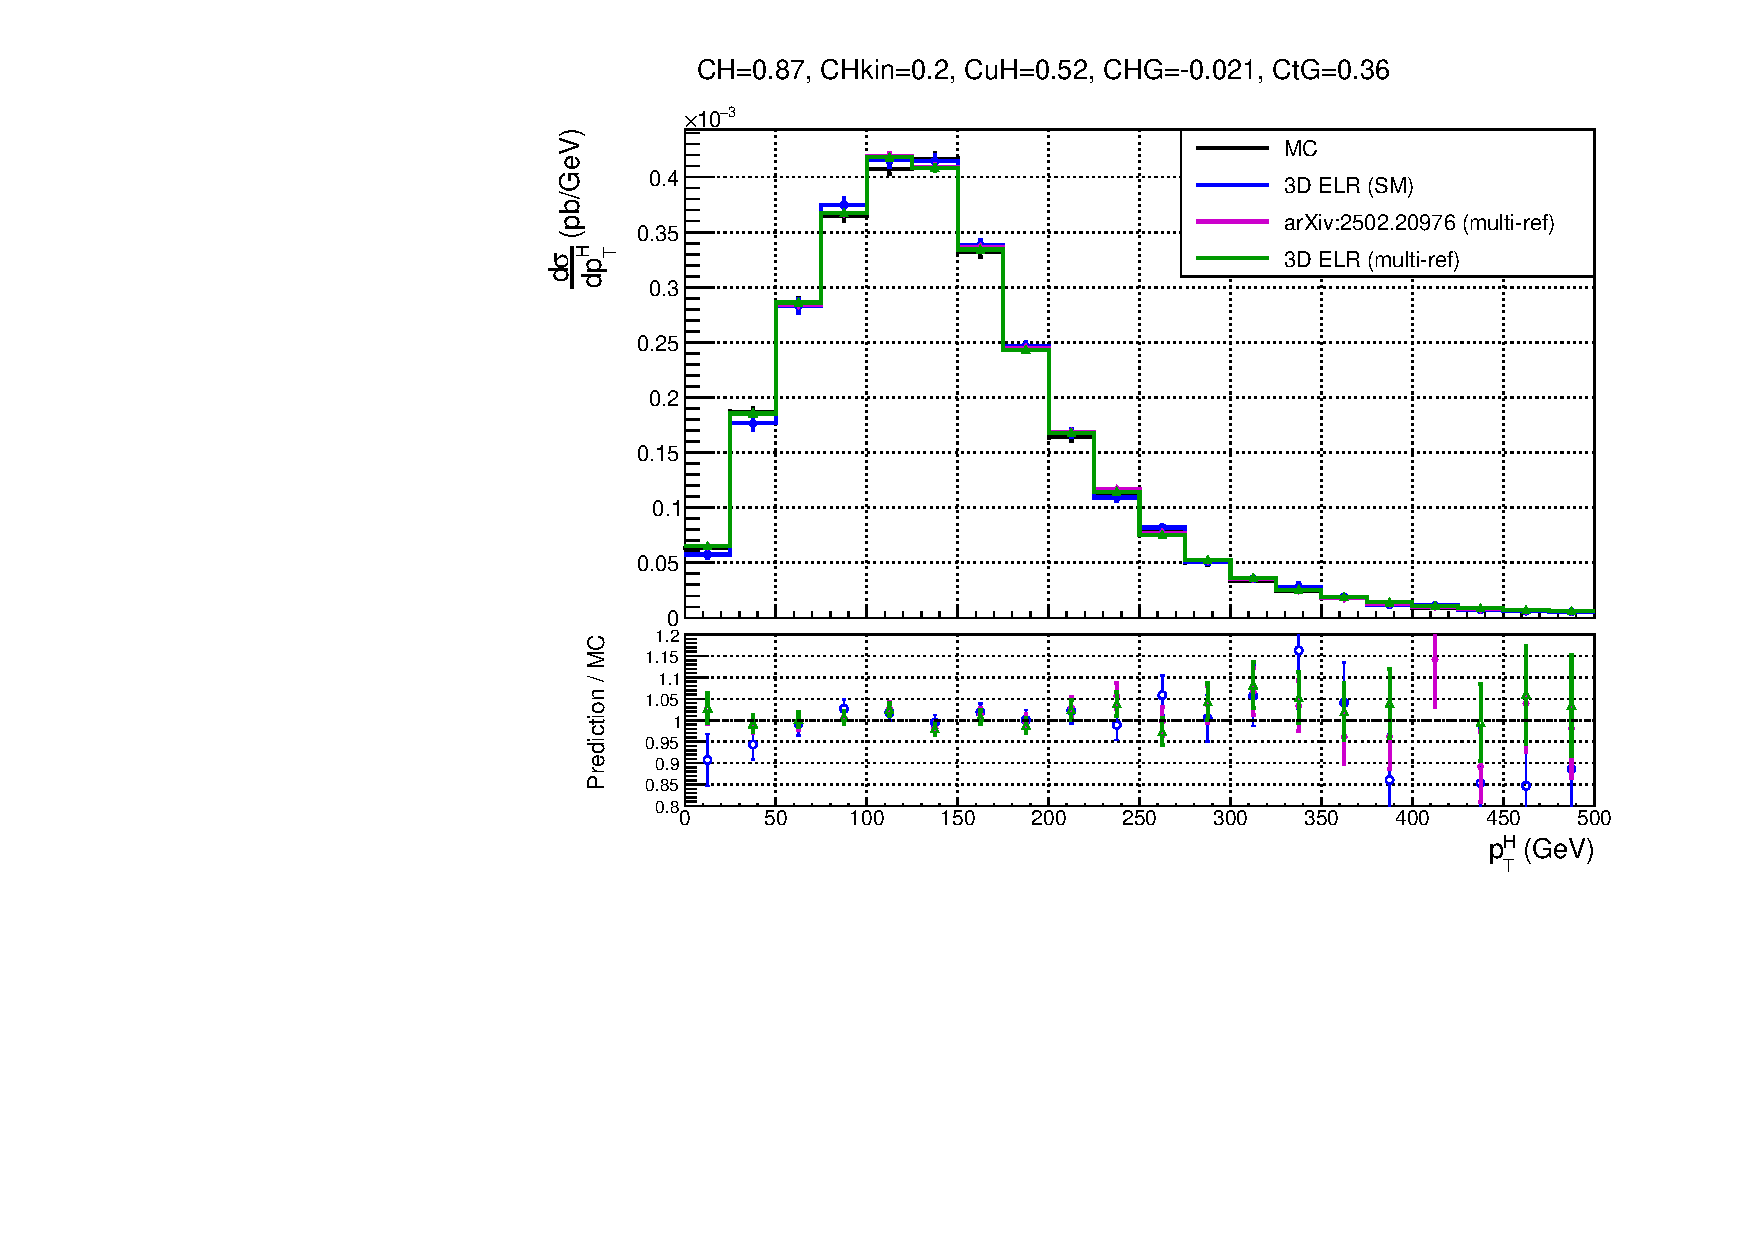
\includegraphics[width=\linewidth]{plots/pth_3d_SM_vs_multiref_vs_Luca_(71)_CH_0.874886_CHbox_0.201155_CuH_0.515566_CHG_-0.0206212_CtG_0.360217_CQt_0.0_CQt8_0.0_CQQtt_0.0_CQQ8_0.0.pdf}
  \end{minipage}
  \hfill
  \begin{minipage}[b]{0.495\linewidth}
    \centering
    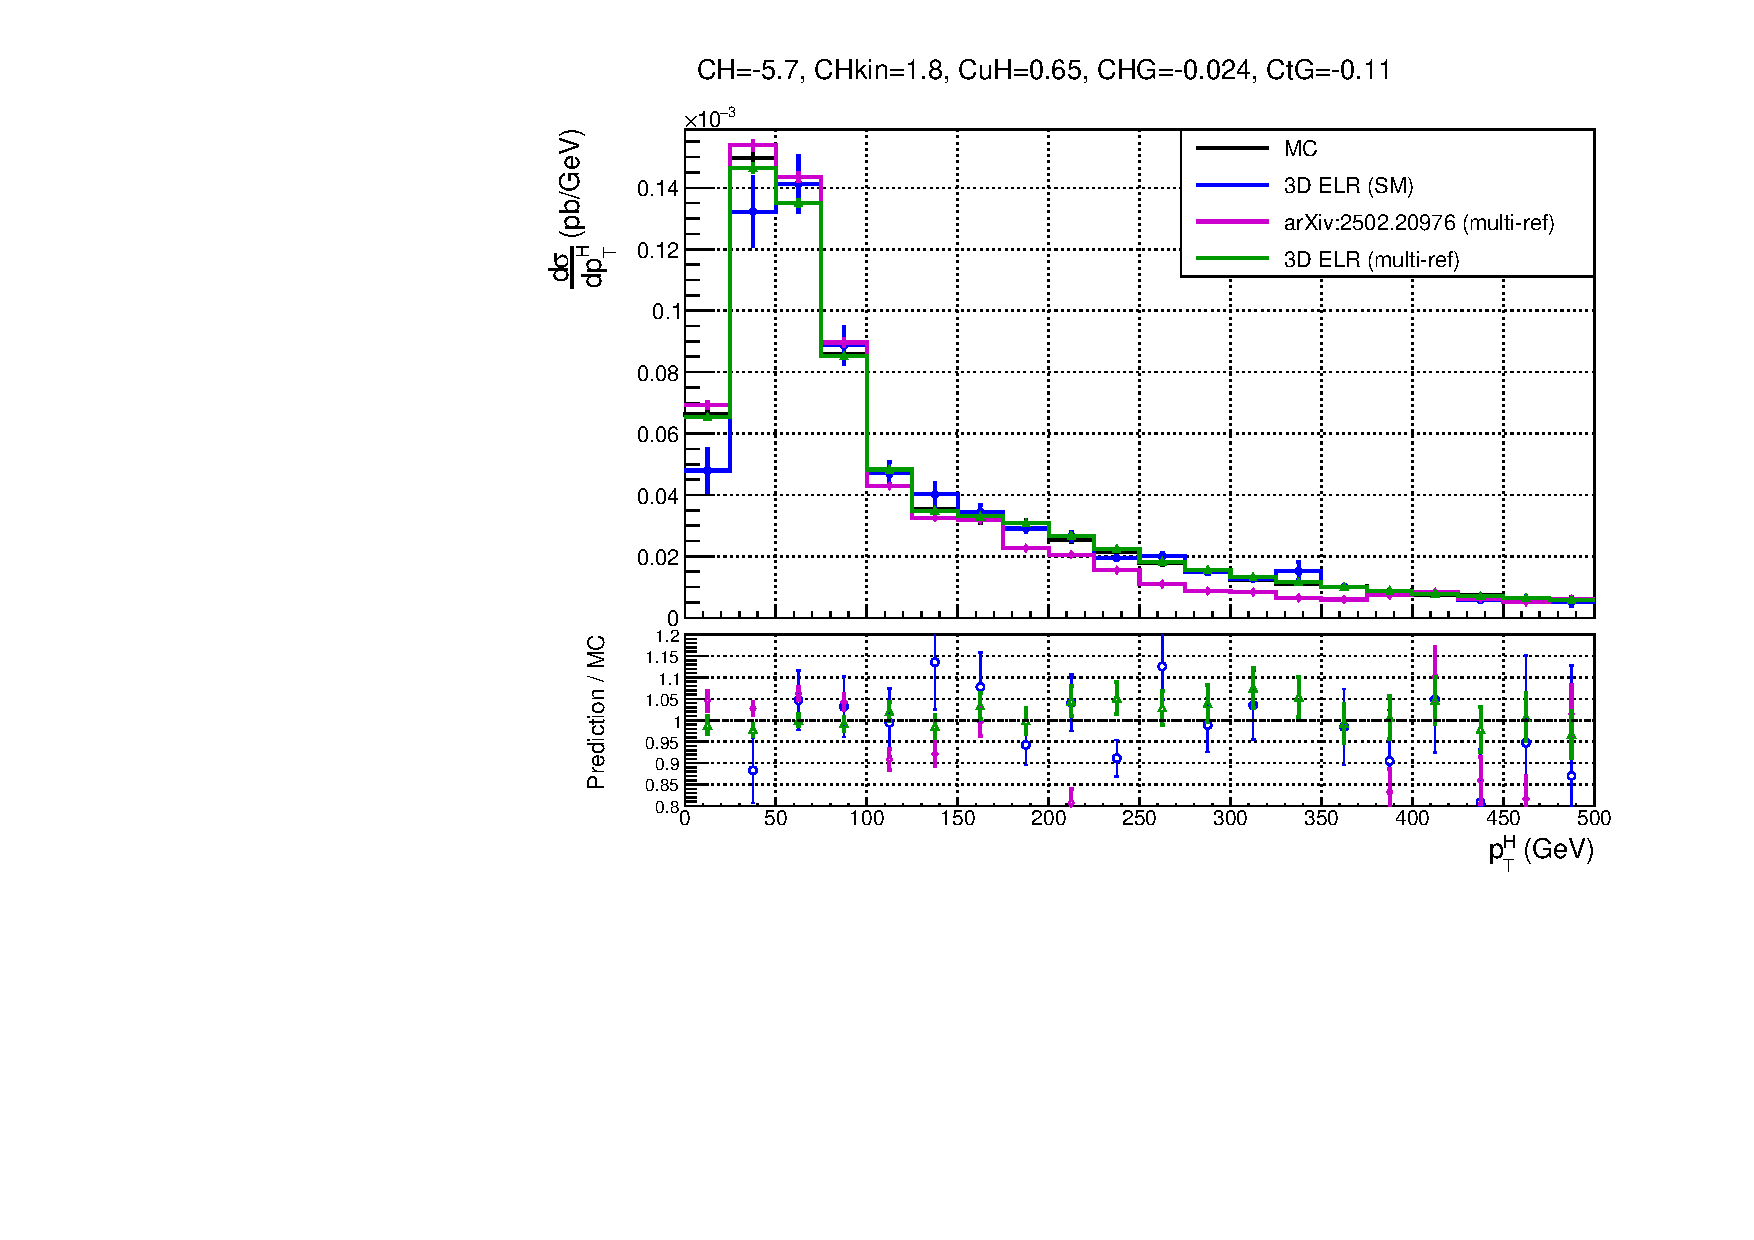
\includegraphics[width=\linewidth]{plots/pth_3d_SM_vs_multiref_vs_Luca_(19)_CH_-5.72209_CHbox_1.76334_CuH_0.653559_CHG_-0.0238598_CtG_-0.10625_CQt_0.0_CQt8_0.0_CQQtt_0.0_CQQ8_0.0.pdf}
  \end{minipage}
  \vspace{0.5em}
  \begin{minipage}[b]{0.495\linewidth}
    \centering
    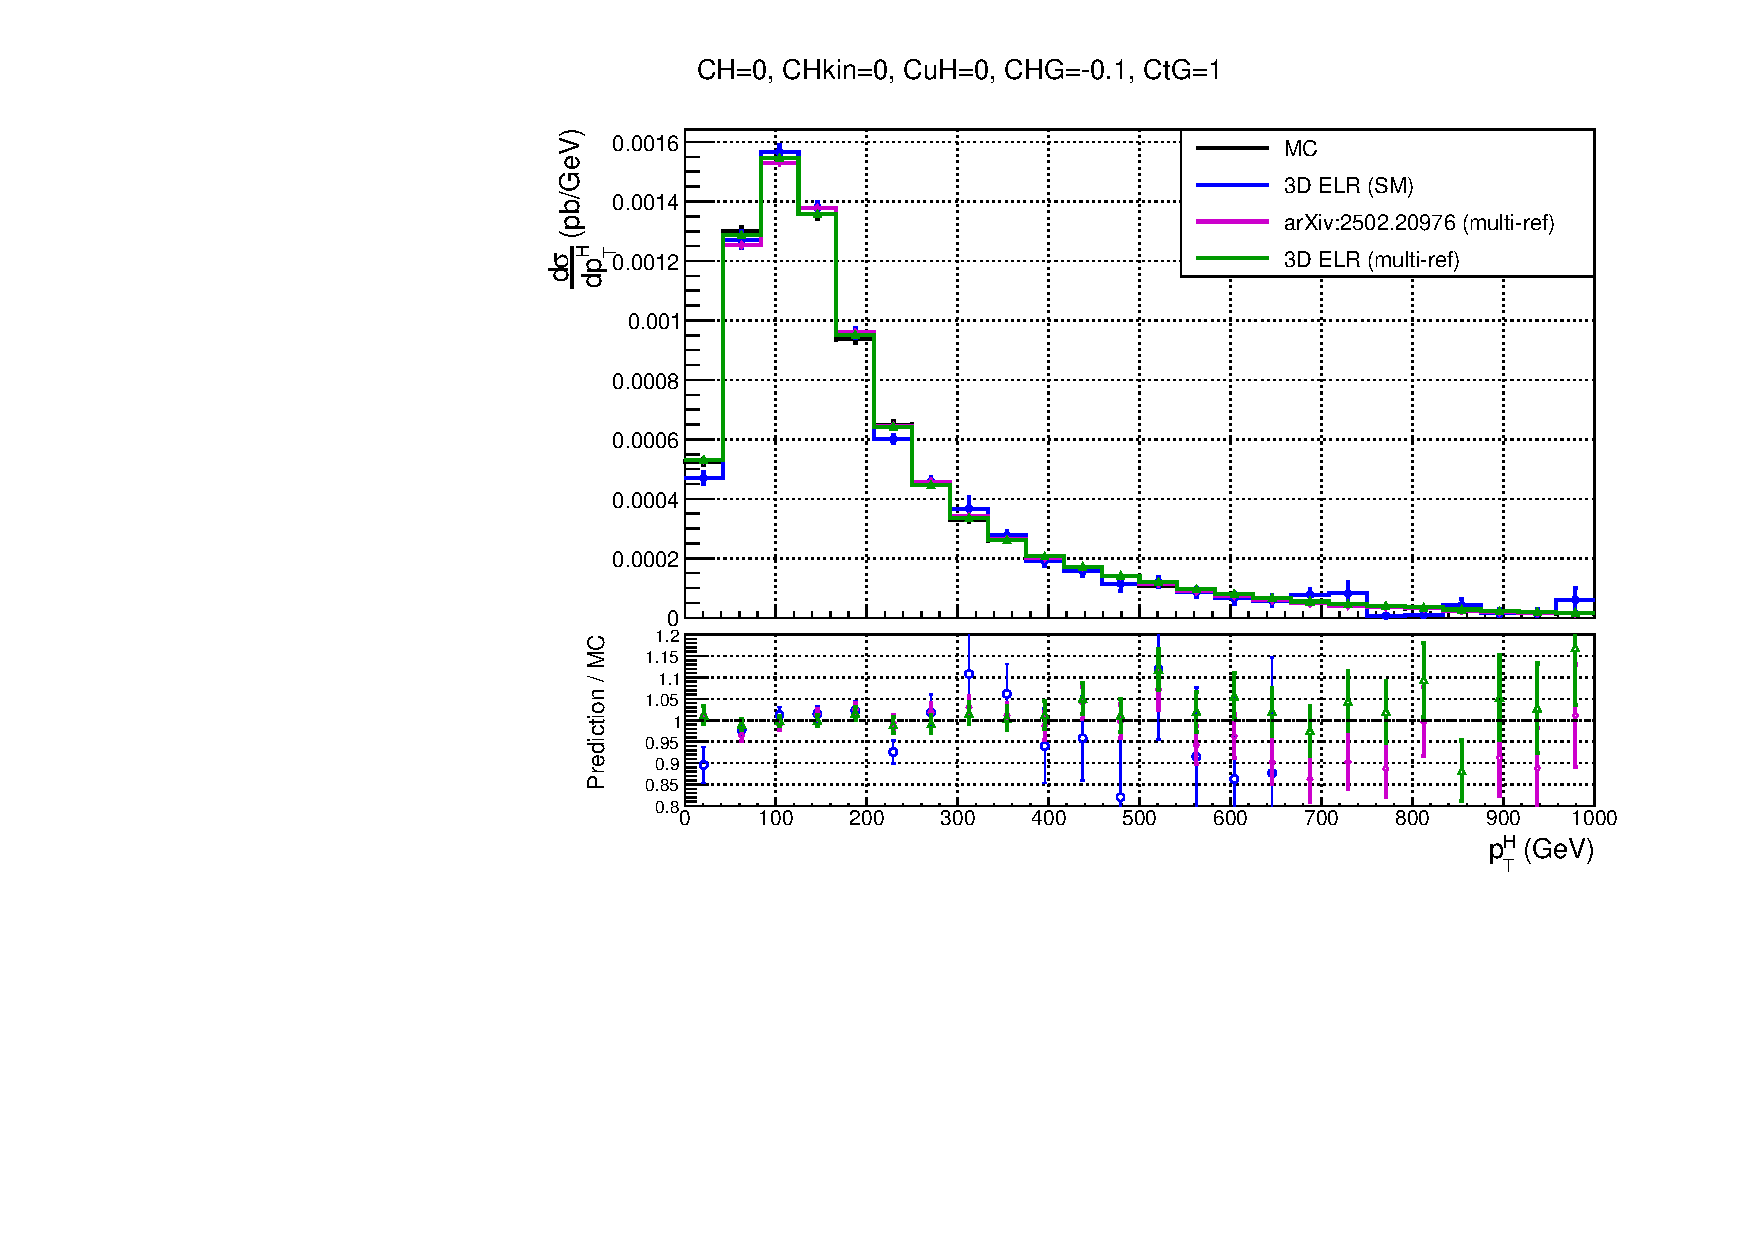
\includegraphics[width=\linewidth]{plots/pth_3d_SM_vs_multiref_vs_Luca_(30)_CH_0.0_CHbox_0.0_CuH_0.0_CHG_-0.1_CtG_1.0_CQt_0.0_CQt8_0.0_CQQtt_0.0_CQQ8_0.0.pdf}
  \end{minipage}
  \hfill
  \begin{minipage}[b]{0.495\linewidth}
    \centering
    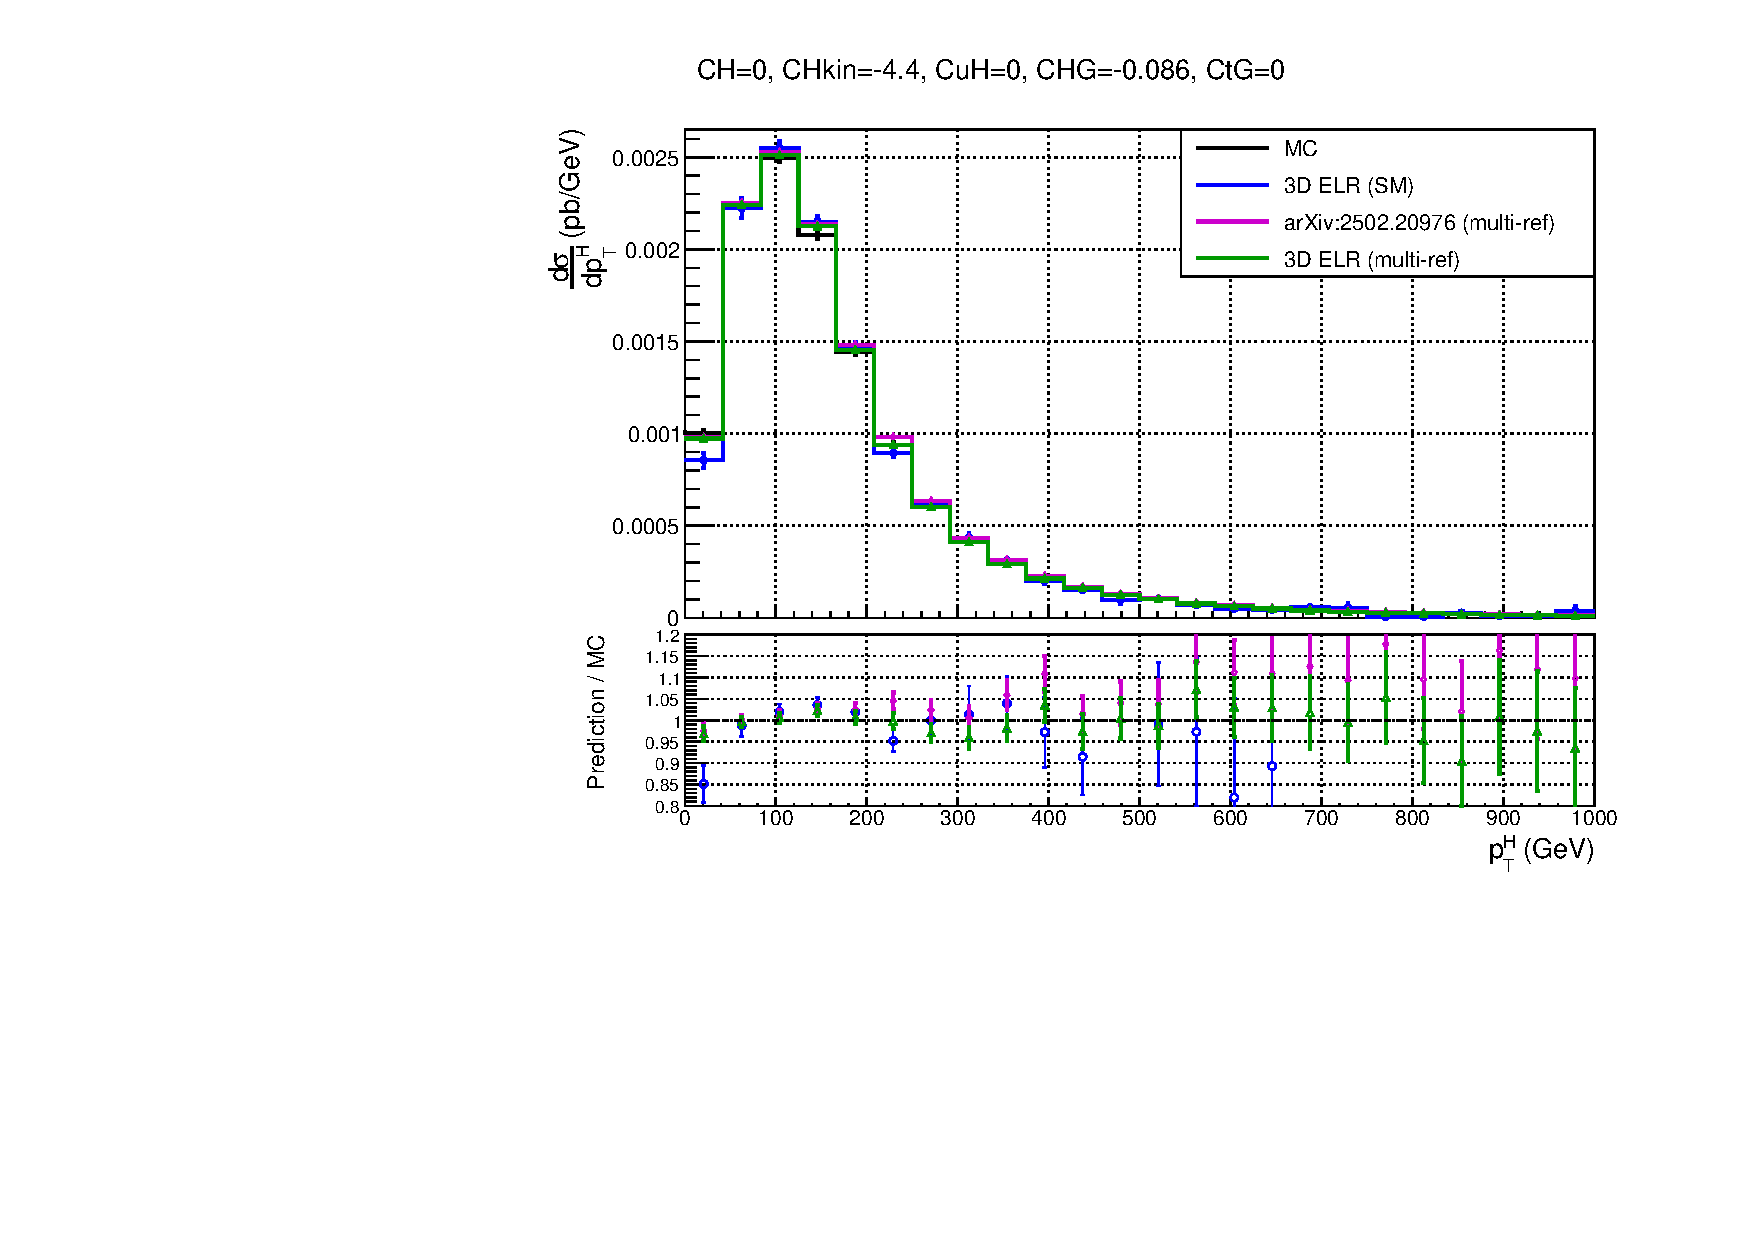
\includegraphics[width=\linewidth]{plots/pth_3d_SM_vs_multiref_vs_Luca_9_CH_0.0_CHbox_-4.44444_CuH_0.0_CHG_-0.0855556_CtG_0.0_CQt_0.0_CQt8_0.0_CQQtt_0.0_CQQ8_0.0.pdf}
  \end{minipage}
  \caption{Some of the test-samples probing the $\{c_\PH,\,c_{\PH \mathrm{kin}},\,c_{u\PH},\,c_{\PH G},\,c_{\PQt G}\}$ subspace. 3D ELR (multi-ref) shows stable modeling in the whole parameter space, also improving the precision in the boosted region, as indicated by the bottom plots.}
  \label{fig:pth}
\end{figure}
\begin{figure}[h!]
    \centering    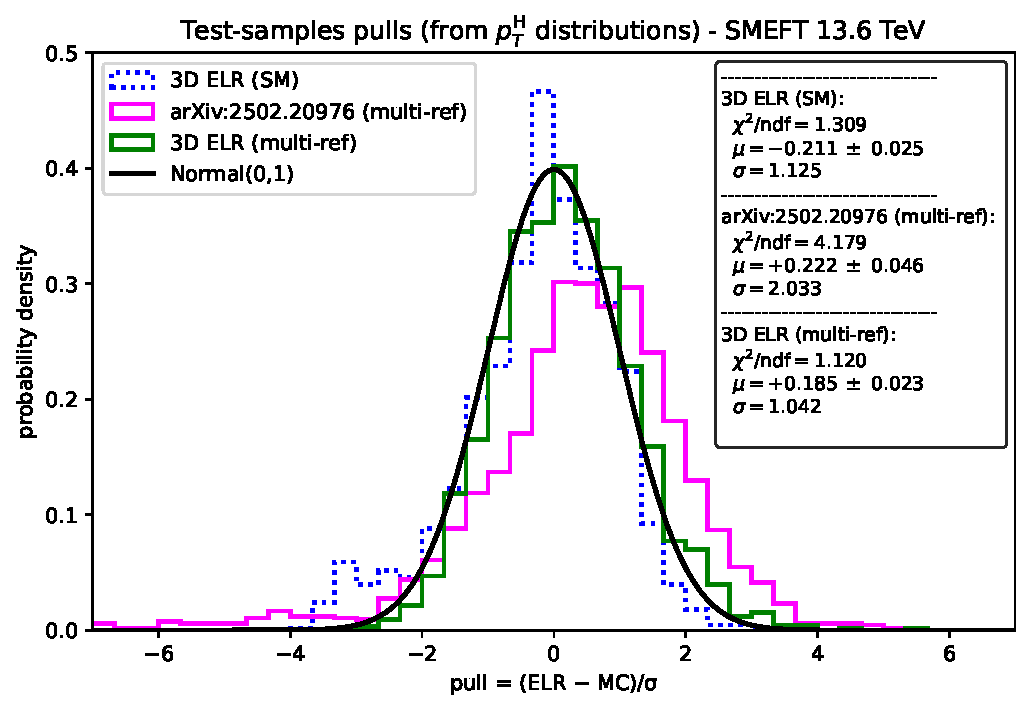
\includegraphics[width=0.8\linewidth]{plots/combined_pth_3d_SMEFT_test_plot_multiref_LUCACOMP_50_1.pdf}
    \caption{Pull distribution and statistical parameters obtained using all test-samples in all $p^\text{H}_T$ bins in SMEFT. We show the $\chi^2_\text{red}$, and the mean ($\mu$) calculated from all pulls, with its error given by $\sigma/\sqrt{N}$, for $\sigma$ the corresponding standard deviation.}
    \label{fig:stats}
\end{figure}
%Two parameterizations are provided: a 1D one differential in \mHH, and a 3D one differential in $\{m_{hh},|\cos\theta^*|,p^{hh}_T\}$. The 1D formula gives the best description of the \mHH shape itself, while the 3D one is the appropriate choice when other kinematic variables have to be reweighted, or when the shape is built after experimental selections, since $p^{hh}_T$ encodes the non-linear effects that such selections induce.

%Independently of the binning, the $A$-coefficients are extracted for two operator sets, from the two grids of Sec.~\ref{sec:grids}. The \emph{9D} parameterization determines all 40 coefficients of Eq.~\eqref{eq:smeftpara_reorg} from the 9D grid and is the \textbf{nominal} result: it is complete, in that it remains valid when the four-fermion operators are switched on, and it is the more stable of the two, the full operator space being populated by the samples. The \emph{5D} parameterization is a reduced fit that keeps only the leading operators together with $c_{\PQt G}$---i.e. the coefficients $A^j_0$--$A^j_{14}$ and the $c_{\PQt G}$ entries of the linear and mixed brackets, with the remaining subleading coefficients set to zero---and is extracted from the 5D grid. It is provided \emph{only for comparison studies}: it is used to check that restricting the operator space leaves the leading coefficients and the reweighted \mHH shapes statistically compatible with the nominal determination, and it does not enter the central results. The comparison of the two is reported in Sec.~\ref{sec:validation}.

%The binning used to extract the formulas is given in Table~\ref{tab:binedge}. As in the HEFT case, the 3D binning is used only in the low-mass region ($m_{hh}<1000$~GeV) and a 1D binning is kept above it, where the number of events per bin would otherwise become too small.

%For the 1D coefficients a per-bin weighted least squares (WLS) fit is used, with every sample having at least one entry in a given bin contributing. For the 3D coefficients the weights are clipped to lie between $0.001$ and $100$ times the median weight of the corresponding bin, which prevents the highest-statistics samples from dominating and washing out the regions where the destructive interference between diagrams is strongest. The motivation and the comparison against the unclipped and iterative alternatives are given in Ref.~\cite{ELR_R5}.


%The $A$-coefficients are extracted independently at each of the three centre-of-mass energies, since the parameterization is a statement about cross sections and the coefficients absorb the energy dependence of the process. Figures in this report show the $13.6$ and $100$~TeV results; the $13$~TeV ones are close enough to the $13.6$~TeV ones that showing them adds nothing, and are provided with the ancillary material.


\subsection{Implementation in the \texttt{ELReweighter}}
\label{sec:elr_implementation}


All the coefficients derived in this work are included in the \texttt{ELReweighter} package presented in Ref.~\cite{ELR_R5}. The tool allows for the ELR of any target point in the SMEFT 9D parameter space. For a given input sample "i", the following weight can be used for building any differential distribution:
\begin{equation}\label{ELReweighter}
    w_i=\frac{Poly(\mathbf{c}^{\text{target}}, \mathbf{A}^j)}{Poly(\mathbf{c}^{\text{input}}_i, \mathbf{A}^j)},
\end{equation}
where $j$ corresponds to a given bin among those shown in Table~\ref{tab:binedge}. The propagated uncertainties consider the statistical error of the input sample and the covariance matrix of the $A$-coefficients. The multi-ref approach is integrated in the \texttt{ELReweighter}, thus several input samples can be used at once. Each provides an estimate of the target distribution from its own events, and the estimates are combined bin-by-bin with weights given by the inverse of their statistical variance, so that every input contributes where its \mHH spectrum is populated.

Any input sample can be used provided the generator-level weights, the HH kinematics and the total cross section are given. The \texttt{ELReweighter} also supports HEFT, therefore HEFT samples can be used as input samples---i.e. the denominator in equation \eqref{ELReweighter}---to generate SMEFT distributions, and vice-versa. In particular, the templates of Sec.~\ref{sec:validation_realistic} are produced this way: four samples generated at different values of $\kappa_\lambda$, in HEFT, supply the whole nine-dimensional SMEFT space. 


%In particular, for investigating both ELR and the matrix method---to be discussed in the next Sections---in SMEFT and in the signal region of recent Run 3 measurements, we refer to the information released by the CMS Run 3 \HH$\to b\bar b b\bar b$ search \cite{CMS:2026znu}, available in the HEPData format \cite{hepdata.171917,Maguire:2017ypu}. The material contains all the experimental selections applied to generator-level events, for four $\kappa_\lambda$ scenarios: $\kappa_\lambda=0,\,1,\,2.45,\,5$. This is done separately for two of the topologies explored in the search, namely resolved, and merged. While the former targets the regime where the four $b$-quarks can be individually reconstructed without overlapping, the latter aims the case where the $b$-jets are produced highly collimated, therefore leaving two large merged jets in the calorimeter. The distributions are used as input to the \texttt{ELReweighter} tool, and are further used 

%the templates of Sec.~\ref{sec:validation_realistic} are produced this way: four samples generated at different values of $\kappa_\lambda$, in HEFT, supply the whole nine-dimensional SMEFT space






%Every result of this report that involves a selection---the acceptance scans of Sec.~\ref{sec:validation_realistic} and the templates the matrix method is built on---is produced with it.
%The coefficients of this section are released in the \texttt{ELReweighter} package of
%Ref.~\cite{ELR_R5}, together with the application recommended here. That package is the
%same one the HEFT report uses; what changes is the parameterization it is given, not the
%machinery. As in Ref.~\cite{ELR_R5} for HEFT, the recommended use is \emph{multi-reference}:
%several input samples reweighted to the same target and combined, rather than one. The
%evidence for that recommendation, and the number of inputs it takes, are in
%Sec.~\ref{sec:validation_nsamples}.

%The tool turns
%an existing simulated sample into a prediction at an arbitrary coupling point by
%reweighting it event by event. The weight of an event is the ratio of the differential
%cross section at the target point to that at the point the sample was generated at,
%evaluated in the $(\pt^{\HH}, |\cos\theta^*|, \mHH)$ cell the event falls in,
%
%\begin{equation}
%w(e) = \frac{\sigma_{\text{t}}(\mathbf{c}_{\text{t}};\,\text{cell}(e))}
%            {\sigma_{\text{in}}(\mathbf{c}_{\text{in}};\,\text{cell}(e))} ,
%\label{eq:elr_weight}
%\end{equation}
%
%with $40$ \mHH bins times the $\pt^{\HH}$ and $|\cos\theta^*|$ bins of
%Table~\ref{tab:binedge}, $1090$ cells in total. The normalization of each input sample is
%taken from its own metadata, as the generator weight times the sample cross section
%divided by the sum of generator weights.

%The input samples need not be generated in the model of the targets. The numerator of
%Eq.~\eqref{eq:elr_weight} is taken from the SMEFT parameterization of this report and the
%denominator from the parameterization of the model the sample was produced in, both
%fitted on the same cells. An input is read in its own couplings only: it is never placed
%in the SMEFT space, and no relation between the coupling modifiers of one model and the
%Wilson coefficients of the other is used. The reweighting uncertainty is that of the
%numerator, propagated from the covariance of the SMEFT coefficients.

%Several input samples can be used at once. Each provides an estimate of the target
%distribution from its own events, and the estimates are combined bin by bin with weights
%given by the inverse of their statistical variance, so that every input contributes where
%its \mHH spectrum is populated. The templates of
%Sec.~\ref{sec:validation_realistic} are produced this way: four samples generated at
%different values of $\kappa_\lambda$, in the $\kappa$ framework, supply the whole
%nine-dimensional SMEFT space.

%The procedure is validated against the one point for which a generated SMEFT sample
%exists. After the resolved $\HH\to\bbbar\bbbar$ selection the SM prediction
%built from the four inputs gives an acceptance times efficiency of $6.06\%$, against
%$6.05\%$ for the generated SM sample histogrammed directly. Each input taken
%alone reproduces the same template to within $1\%$ for $\kappa_\lambda = 0$ and $2.45$ and
%$4\%$ for $\kappa_\lambda = 5$, the last reflecting that the stated cross section of that
%sample is $4\%$ higher relative to the $\kappa$ parameterization than the others'. A
%further check is available to any analysis using this procedure: the SM point
%of a SMEFT table has to agree with the SM point of a $\kappa$ table built from
%the same inputs, since the two describe the same physical point and the second is reached
%without the SMEFT reweighting.